\newtheorem{defn}{Definition}[section]
\newtheorem{exmp}{Example}[section]
\chapter{Methodology}
Elliptic curve cryptography was discovered in 1985 by Victor Miller and Neil Koblitz as an Elliptic Curve Method (ECM) was applied on cryptography known as Elliptic Curve Cryptography.
Cryptography based on Elliptic Curves (ECC) has the unique feature of being the finest up to now.It can be solved using a well-known approach that takes full exponential time to complete.The Elliptic Curve Logarithm is responsible for its safety.In a group specified by the Discrete Logarithm Problem (DLP) over a finite field, using points on an elliptic curve,To attain the same level of security as traditional public key cryptography techniques, the required key size must be drastically reduced.As a result of that,an appropriate public key scheme would be one that is cost-effective in terms of compute and key sizes,Compared to other public key cryptosystems, ECC offers the highest strength-per-bit. The smaller the key, the less bandwidth, memory, and processing power are used.\\
\section{Group Law}
We first consider the case of Weierstrass
elliptic curves. Let $L$ be a line, with the following rules:
\begin{enumerate}
	\item 	The identity element is 0 = [0 : 1 : 0].
	\item	If $A$, $B$, $C$ are 3 distinct points of  $ L \cap E$  then $A+B+C=0$.
	\item	If $ L \cap E$ consists of exactly 2 points $A$ and $B$, and $L$ is tangent to $E$ at $A$, then $A + A + B = 0$.
	\item	If $ L \cap E$ is just a single point $A$ and $L$ is tangent to $E$ at $A$, then we
	have $A + A + A = 0$.\\
It is commonly known that when the points on an elliptic curve are added together, they form an abelian group. Let $E$ be the Weierstrass equation for an elliptic curve.	
\end{enumerate}
\subsection{Weierstrass Equation}
Weierstrass equation is given as;
\begin{equation}
		Y^2 = X^3 + aX + b
\end{equation}
The addition rule is given below:
For all $P,Q,E$\\
(i) $O+P = P$ and $P+O = P$. (So O serves as the identity element.)\\
(ii) -O = O.\\
(iii) If P = ($x_{1},y_{1}$) :f: 0, then -P = ($x_{1}, -y_{1} - a_{1}x_{1} - a_{3}$). (Note
that $P$ and $-P$ are the only points on $E$ with x-coordinate equal to $X_{1}$\\ (iv) If $Q=-P$, then $P+Q =O$.\\
(v) If $P \neq O , Q\neq O , Q\neq-P$, then let $R$ be the third point
of intersection (counting multiplicities) of either the line $\overline{PQ}$ if
$P \neq Q$, or the tangent line to the curve at $P$ if $P = Q$, with
the curve (as usual, the tangent line to the curve $f(x, y)=0$ at
$P = (a,b)$ is the line $\frac{\partial{f}}{\partial{x}}(P)(x-a)+\frac{\partial{f}}{\partial{y}}(P)(y-b)$= 0. Then $P+Q = -R$\\\\

\subsection{Group Properties}
Elliptic curves are the set of points that are obtained as a result of solving an elliptic curves function over a predefined space.\\
{\bf Definition:}\\
An elliptic curve over $K$ is a nonsingular projective algebraic curve $E$ of genus 1 over $K$ with a chosen base point o in $E$.\\
{\bf Some points in elliptic curve:}\\ 
$\bullet$ Elliptic curves have point with coordinated in any finite field that is rational point, real point, complex point and finite point.\\
$\bullet$	Elliptic curves with point with point in $F_{p}$ are finite group.

\begin{figure}[h]
	\centering
	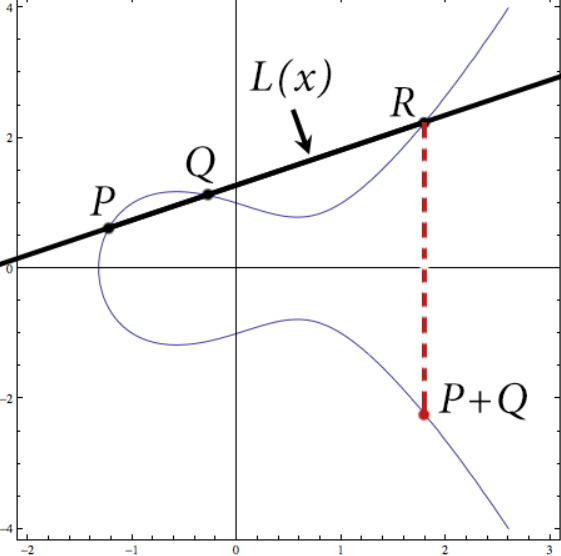
\includegraphics[scale=0.5]{project.jpg}
	\caption{Geometric figure of an Elliptic curve}
	\label{fig:project}
\end{figure}

\section{Using one solution to find various solution to an elliptic curve}
The elliptic curve is defined by a certain type of cubic equation with two variables.
The set of rational solutions to the equation has an extremely interesting structure, including the group law.\\\\

{\bf Taking the figure below:}\\
\begin{figure}[h]
	\centering
	\includegraphics[width=0.7\linewidth]{diagram 1}
	\caption{}
	\label{fig:diagram-1}
\end{figure}
We are to find all the point of on the figure below,and doing so we first find the values of $a$ and $b$\\
Finding the value of $a$ and $b$\\
Given:\\
Let $Y = 0$\\
$0^{2}-0=x^{3}-x$\\
$x(x+1)(x-1)=0$\\
From here, $a=-1$ and $b=1$\\
Find the values of $\delta$\\
Adding $\frac{1}{4}$\\
$Y^{2}-Y+\frac{1}{4}=X^{3}-X+\frac{1}{4}$\\
$(Y-\frac{1}{2})^{2}=X^{3}-X+\frac{1}{4}$\\
From $(Y-\frac{1}{2})^{2}=X^{3}-X+\frac{1}{4}$,\\
$\delta = \frac{1}{2}$\\
Why the curve is symmetric about Y=$\delta$\\
$(Y-\frac{1}{2})^{2}=X^{3}-X+\frac{1}{4}$\\
$Y=\frac{1}{2}\pm{\sqrt{X^{3}-X+\frac{1}{4}}}$\\
Note: if $\left(X,\frac{1}{2}+{\sqrt{X^{3}-X+\frac{1}{4}}}\right)$ is on the curve, so is the point $\left(X,\frac{1}{2}-{\sqrt{X^{3}-X+\frac{1}{4}}}\right)$.\\
\begin{figure}[h]
	\centering
	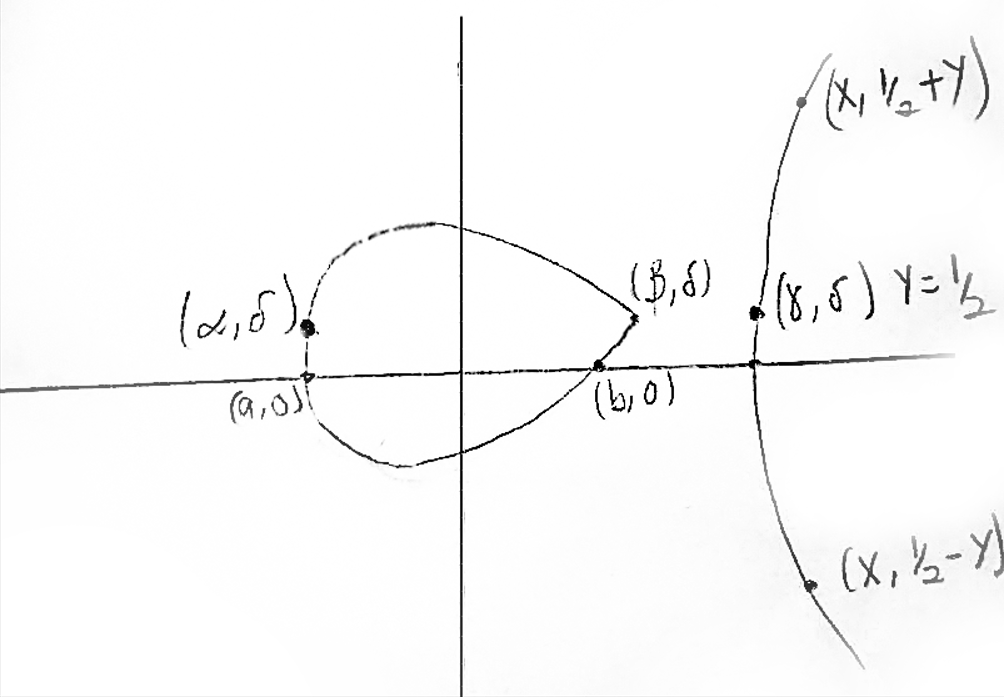
\includegraphics[width=0.7\linewidth]{Diagram 2}
	\caption{}
	\label{fig:diagram-2}
\end{figure}
Finding a cubic equation with roots $\alpha, \beta, \gamma$\\
Taking the second line obtained from the object to be our x-axis\\
Let $Y = \frac{1}{2}$\\
$\left(\frac{1}{2}-\frac{1}{2}\right)^{2}=X^{3}-X+\frac{1}{4}$\\
$X^{3}-X+\frac{1}{4}=0$\\
Find $\alpha+\beta+\gamma$\\
$X^{3}-X+\frac{1}{4}=(X-\alpha)(X-\beta)(X-\gamma)$\\
$X^{3}-X+\frac{1}{4}=X(X^{2}-(\alpha+\beta)X+{\alpha}{\beta}(X-\gamma)$\\
$X^{3}-X+\frac{1}{4}=X^{3}-(\alpha+\beta+\gamma)X^{2}+...$\\
$X^{3}-X+\frac{1}{4}= - (\alpha+\beta+\gamma)=0$\\
$\alpha$+$\beta$+$\gamma=0$\\\\
Let C be the circle with ($\alpha$, $\delta$),($\beta$,$\delta$) as ends of a diameter.\\
Equation of a circle: $a^{2}+b^{2}=r^{2}$\\
Put the centre \big($\frac{\alpha+\beta}{2},\frac{1}{2}$\big) into the equation of a circle\\
\begin{figure}[h]
	\centering
	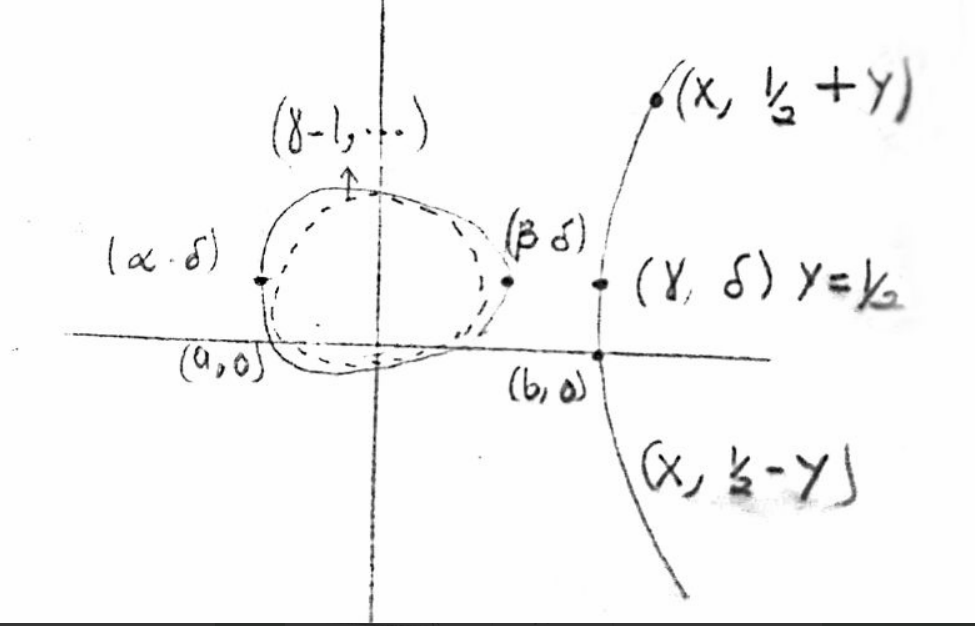
\includegraphics[width=0.7\linewidth]{Diagram 3}
	\caption{}
	\label{fig:diagram-3}
\end{figure}
Centre $\big(\frac{\alpha+\beta}{2},\frac{1}{2}\big)$\\
$\big(X-\frac{\alpha+\beta}{2}\big)^{2}+\big(Y-\frac{1}{2}\big)^{2}=\big(\frac{\beta-\alpha}{2}\big)^{2}$\\
Showing that C intersect S at two other points and finding the X-coordinate in terms of $\delta$\\
$\big(X-\frac{\alpha+\beta}{2}\big)^{2}+X^{3}+X-\frac{1}{4}=\big(\frac{\beta-\alpha}{2}\big)^{2}$\\
Note we know that $\alpha$ and $\beta$ are solutions to $\big(X-\frac{\alpha+\beta}{2}\big)^{2}+X^{3}+X-\frac{1}{4}=\big(\frac{\beta-\alpha}{2}\big)^{2}$ ,let S be the $3^{rd}$ solution\\
Since the coefficient of $X^{2}$ in $\big(X-\frac{\alpha+\beta}{2}\big)^{2}+X^{3}+X-\frac{1}{4}=\big(\frac{\beta-\alpha}{2}\big)^{2}$  is 1\\
So $\alpha+\beta+S=-1$\\
${-\gamma+S}=-1\\
$S=$\gamma$-1\\
\section{Finding point algebraically}
For any points $P$ and $Q$ on an elliptic curve, EC group law point addition can be used geometrically to find various points in the plane. If we draw a line through $P$ and $Q$, this line will intersect the elliptic curve at a third point (-R). The reflection of this point about x-axis, $R$ is the addition of $P$ and $Q$.\\
Bezout's Theorem establishes that the intersection of $P$ and $Q$ is valid and it states; Suppose that X and Y are two plane projective curves defined over a field F that do not have a common component (X and Y are defined by polynomials whose greatest common divisor is a constant). Then the total number of intersection points of X and Y with coordinates in an algebraically.
The closed field $E$, which contains $F$, counted with multiplicity, is equal to the product of the degrees of $X$ and $Y$. This makes the formation of the third point $R$ after the intersection of $P$ and $Q$.\\
{\bf Properties}
\begin{enumerate}
	  \item If a line intersects two points, it intersects a third. 
	  \item If a line is tangent to the curve, it intersects another point.
	  \item All vertical lines intersect the point at infinity.
      \item The curve has an ever-increasing slope after a point of inflection.\\
\end{enumerate}
{\bf The Addition Law}\\
The curve E under the point of addition is an abelian group with these properties:
\begin{enumerate}
    \item Identity-at infinity
	\item Inverse-the reflection of a point.
	\item Associativity
	\item commutativity
\end{enumerate}
\begin{figure}
	\centering
	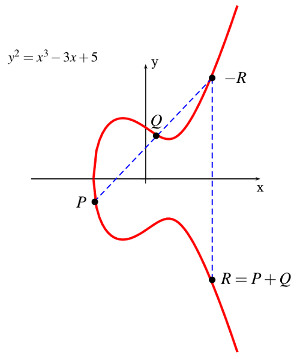
\includegraphics[width=0.7\linewidth]{nkLWe}
	\caption{}
	\label{fig:nklwe}
\end{figure}
First step in finding the equation is to define the line.\\
$P=(X_{1},Y_{1})$ and $Q=(X_{2},Y_{2})$\\
$\bullet$ The point-slope from the line.\\
$\lambda$=$\frac{y_{2}-y_{1}}{x_{2}-x_{1}}$\\
$y-y_{1}$ =  $\lambda$  $(x - x_{1})$\\
$\bullet$ The slope-intercept form of the line.\\
$y$= $ \lambda$x - $\lambda$ $x_{1} + y_{1}$\\
$\beta$= $y_{1}$ - $\lambda$ $x_{1}$\\
$y= \lambda $x$ + \beta$\\
Finding $x_{3}$ and $y_{3}$ of points 3\\
y=$\lambda$ $x$ + $\beta$\\
squaring both sides\\
$y^{2}$ = $( \lambda $x$+ \beta )^{2}$\\
The curve $y^{2}$ = $x^{3}+ax+b$\\
$( \lambda $x$ + \beta)^{2}$ = $x^{3}+ax+b$\\
$0={x^{3}}-\lambda^{2}{x^{2}}-2{\lambda}{x}{\beta}-{\beta^{2}}$+{ax+b}$\\
${${{x}_{1}}$,${{x}_{2}}$,${{x}_{3}}$}$\,\,{\textit{are the roots.}} \\
${$({{x}_{1}}+{{x}_{2}}+{{x}_{3}})={{\lambda}^{2}}$}$\\ 
x_{3}= \lambda^{2}-x_{1}-x_{2}\\
y_{3}= \lambda (x_{1}-x_{3}) -y_{1}\\
$ 
\subsection{Identity}
{\bf Definition:}\\
Let $P$ be the elliptic curve $E$, and $O$ be the point at infinity,then $P$+$O$=$O$ + $P$
Finding the point at infinity 0\\
\begin{enumerate}
	\item Adding infinity results in a vertical line.
	\item Then find the third point of intersection.
	\item After the reflection the result turns to be the original point.
\end{enumerate}
$P+\infty =P$

The figure below illustrate this concept: 
\begin{figure}[h]
	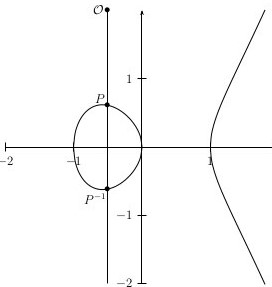
\includegraphics{identity.image}
	\caption{}
	\label{fig:identity}
\end{figure}
\subsection{Inverse}
An operation (+) is said to be invertible within a set if each element P has an element with the same set $P^{-1}$ such that $P+P^{1}=O$ where O is the identity of the operation within the set.In this case,P and $P^{-1}$ are said to be inverses of each other. \\\\
\begin{figure}[h]
	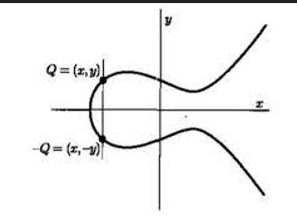
\includegraphics{Screenshot (91)}
	\caption{}
	\label{fig:screenshot-91}
\end{figure}
$P$+$-P$=$\infty$\\
The reflection of a point is it inverse\\
so, if we define\\
$P$=($x$,$y$) and $-P$=($x$,$-y$)\\
$P-P$=$\infty$\\
\subsection{Associative}
An operation is said to be associative if $P+(Q+R)=R+(P+Q)$ for all P,Q,R within a set.The steps used to find the operation of normal addition (+) on associativity on a geometry is below:\\\\
\begin{enumerate}
	\item Taking a line through $P$ and $Q$ we get $P+Q$ and it reflection is $P+Q$.
	\item Taking a line through $P$ and $Q$ we get $P+Q$ and it reflection is $P+Q$.
	\item Taking a line through $Q$ and $R$ we get $Q+R$ and it reflection is $Q+R$.
	\item Taking a line through  $Q+R$ and $P$ it turns $P+(Q+R)$.
	\item Taking a line through  $P+Q$ and $R$ it turns $R+(P+Q)$.
	\item The line  $R+(P+Q)$ and $P+(Q+R)$ intersect at a point whose reflection form a vertical line thus at $\infty$.
	\item This makes $R+(P+Q)$ and $P+(Q+R)$ equal. Taking a line through $Q$ and $R$ we get $Q+R$ and it reflection is $Q+R$.
	\item Taking a line through  $Q+R$ and $P$ it turns $P+(Q+R)$.
	\item Taking a line through  $P+Q$ and $R$ it turns $R+(P+Q)$.
	\item The line  $R+(P+Q)$ and $P+(Q+R)$ intersect at a point whose reflection form a vertical line thus at $\infty$.
	\item This makes $R+(P+Q)$ and $P+(Q+R)$ equal.
\end{enumerate}
\begin{figure}
	\centering
	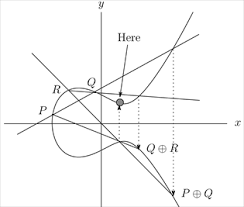
\includegraphics[width=0.7\linewidth]{associative image}
	\caption{}
	\label{fig:associative-image}
\end{figure}
\newpage
\subsection{Point Doubling}
When the points $P$ and $Q$ are of the same coordinates, addition is identical, except there is no well-defined straight line between $P$ and $Q$, so the operation is closed using the limiting case, the tangent to the curve, $E$, at $P$ and $Q$.\\
\begin{figure}
	\centering
	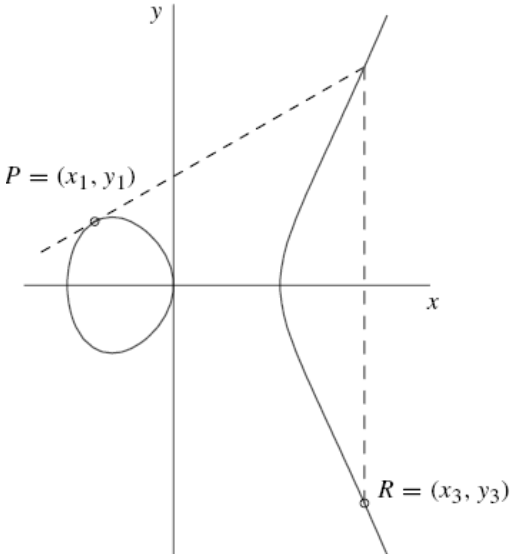
\includegraphics[width=0.7\linewidth]{Screenshot (93)}
	\caption{}
	\label{fig:screenshot-93}
\end{figure}
\newpage
Point doubling is calculated using following equation:\\
$$2P=(x_{3},y_{3})$$,where
$$x_{3}=\lambda^{2}-2x_{1}$$
$$y_{3}=\lambda(x_{1}-x_{3})-y_{1}$$
$$\lambda=\frac{3x_{1}^2+a}{2y_{1}}$$
Thus:if $P=Q$\\\\The properties of the group law all works together for good for elliptic curve cryptography.It basically works good under the addition law and point doubling,in elliptic curve cryptography.This makes the security of elliptic curve cryptography more reliable because a series of generator points has to be traced back to the original point, and it will be very difficult to do so based on the repeated point addition and point doubling.\\ 
\section{cyclic group}
Let $G$ be a finite group of order $n$ is called cyclic if there is an identity element $a \in G$ such that the cyclic subgroup generated by $a$ is the entire group G. In other words,
$G = {a^{n}: n \in Z}$.
Such an element a is called a generator of G.\\Note: A cyclic group is abelian but a group that is abelian is not necessarily.\\
To do some work with the points of elliptic curves, you will need to know what an elliptic curve is and what a group law is. The cyclic subgroup, the base point, and the order can be determined using the points of an elliptic curve when they are restricted to finite fields of integers modulo a prime.

\subsection{The Key Pair Generation of ECC}
Elliptic curve cryptography requires the following parameters below:
\begin{enumerate}
\item The finite field's size is specified by the prime $p$.
\item The elliptic curve equation has coefficients a and $b$.
\item The cyclic subgroup is generated by the generator $G$.
\item $n$ is of the subgroup's order.
\end{enumerate}
The private key is a random integer d selected from the range ${1,...,n-1}$, where n is the subgroup order. The public key is $PK=dG$, where $G$ is the subgroup's generator.
Finding $PK$ is simple if we have $d$ and $G$, as well as the other domain parameters. Finding the private key $d$ is difficult if we know $PK$ and $G$ since it requires solving the discrete logarithm issue.
\section{Diffie - Hellman Key Exchange on elliptic curve cryptography}
Suppose Budu-Biney and his Bank establish a common key with his bank with the aim to exchange data as part of symmetric encryption scheme.\\
\begin{enumerate}
\item Budu-Biney and his Bank agree to use a specific curve (elliptic curve E) over a finite field Fq  that makes the discrete logarithm problem impossible in E ($F_{q}$). They all agreed on a point $P\in(F_{q})$ indicating that the P-generated subgroup has a big order.
\item Alice selects a secret  $b$ $\in$ $Z$ and enumerate bP = Pb and sends Pb to  his bank.
\item Bank select a secret $c \in Z$ and enumerate $cP = Pc$ and sends $Pc$ to Budu-Biney
\item Budu-Biney enumerate $bPc = bcP$.
\item The Bank enumerate $cPb = bcP$.
To extract a key from $bcP$, Budu-Biney and his bank utilize a widely accepted approach, such as the final 256 bits of $bcP's$ x-coordinate.	
\end{enumerate}
On the elliptic curve E, the finite field $F_{q}$ and the points $P$, $bP$, and $cP$.The only way an intruder can get Budu-Biney's  secret key is to use $P$, $bP$, and $cP$ to determine $bcP$. If the intruder can find the discrete logs over E($F$), them the intruder could use $P$ and $bP$ to find Budu-Biney's secret key b.Then the third person could now find $b(cP)$ to get $bcP$. Solving discrete logs knowledge is required to solve it and without it is assumed to be infeasible to fine over E($F_{q}$).\\
To determine whether $Q = bcP$ given $P$, $bP$,$cP \in E(F_{q})$ and a point $Q \in E(F_{q})$ in a comparable problem known as the Decision Diffie-Hellman problem. In other words, can you verify that $bcP$ is right. In some situations, as shown below, the Weil pairing can be utilized to solve the Decision Diffie-Hellman issue.
\section{ElGamal Public Key Encryption}
Assume Budu-Biney wants to communicate with his Bank.To begin, the bank creates it public key in the manner described below.The bank selects an elliptic curve E over Fq that makes the discrete logarithm issue for E(Fq) impossible, as well as  point $P \in E(Fq)$ P have a large prime order.The bank also selects a secret $a \in Z$ and calculates $B = aP$. As a result, Budu-Biney's public and private keys are E, Fq, P, and B, respectively.\\To send a message to the bank, Budu-Biney follows the steps below.
\begin{enumerate}
\item The Bank's public key is downloaded.
\item Use a point $M \in E$ to convey her meaning (Fq).
\item He selects a secret $k \in Z$ and calculates $M_{1} = kP$.
\item $M_{2} = M + kB$ is calculated.
\item $M_{1} and M_{2}$ are sent to his bank.
\end{enumerate}
The bank calculates the cipher text in order to decrypt it.
$M_{2}-sM_{1}=(M+kB)-s(kP)=(M+skP)-skP=M$\\
if the intruder has the bank's public key as well as the points $M_{1} and M_{2}$, but there appears to be no way for the intruder to access M  if the intruder  does not know how to solve discrete logs. Budu-Biney must use a different $k \in Z$ each time he sends a message to the bank, which is an essential note about the $k \in Z$ he chooses at random.The intruder can quickly detect Budu-Biney's usage of the same integer k if he computes M and M0 with the same value of k. The bank may then use $M_{2}M_{20} = M_{0}$ to recover the message M by remembering that $M_{0} = M M_{2} + M_{2}$

\section{ElGamal Digital Signatures}
Let's say Budu-Biney wants to sign a bank document electronically. One method is to digitalize Budu-Biney's signature. However, the bank can copy Budu-Biney's digital signature and then attach it to any document. The steps that are required to be used so that such a digital signature can only be used once. However, someone should be able to verify that the signature is genuine and that Budu-Biney is the one who signed the document. One solution to the problem is based on the discrete logarithm problem's difficulty.Budu-Biney first picks an elliptic curve E over a finite field $F_{q}$ in which the discrete logarithm issue is impossible to solve (Fq).He also chooses $A \in E(F_{q})$ as a location where $|A| = N$ is a huge prime.Budu-Biney also selects $a \in Z$ secret and calculates the location $B = aA$. Finally,He selects a function $f: E(F_{q}) \longrightarrow Z$ that has the property of having a huge picture and just a small number of inputs that result in a certain output.As a result, Budu-Biney's public key is composed of the letters $E, F_{q}, f, A, and B$. The secret $a \in Z$ is his private key. The order of point A,On the other hand, it does not have to be made public. As a result, Budu-Biney does the following to sign the bank document:
\begin{enumerate}
\item The bank document is represented as $m \in Z$. If $m > N$, Budu-Biney will select a larger curve.
\item R = kA is solved by picking a random $k \in Z$ and setting $gcd(k, N) = 1$.
\item Solves $s\equiv k^{-1}(m-af(R))(mod N)$
\end{enumerate}
After the message has been signed $(m, R, s)$. It is worth noting that Budu-Biney is not interested in keeping the message m a secret. If he wants to do so, he will need to employ some type of encryption.The bank then confirms that the communication is from Budu-Biney by saying:
\begin{enumerate}
\item The bank downloads Budu-Biney's information
\item Calculates $V_{1} = f(R)B + sR and V_{2} = mA.$
\item If $V_{1} = V_{2}$, then the bank declares that the signature is authentic.
\end{enumerate}
R is the same in both signatures, thus you will have to do it twice. The following are the equations for $s$ and $s^{'}:$
$$ks\equiv(m-af(R))(mod N)$$
$$ks^{'}\equiv(m^{'}-af(R))(mod N)$$
Taking the difference between these two match gives $k(s-s^{'})\equiv(m-m^{'})(mod N)$.Set $d=gcd(s-s^{'},N)$ then there are $d$ possible values of $k$.The intruder tries all of them until he finds R = kA. He can then locate an as previously once he knows k.







